\documentclass{article}
\usepackage[utf8]{inputenc}
\usepackage[letterpaper, margin=1in]{geometry}
\usepackage{graphicx}
\usepackage{enumitem}
\usepackage{amsmath}
\linespread{1.5}
\let\OLDthebibliography\thebibliography
\renewcommand\thebibliography[1]{
  \OLDthebibliography{#1}
  \setlength{\parskip}{0pt}
  \setlength{\itemsep}{0pt plus 0.3ex}
}
\begin{document}

\title{Boosting Higgsino Searches in the ATLAS Detector Through Object Identification Using Neural Nets}
\author{Matt Zhang \\ Advisor: Ben Hooberman}
\date{December 08, 2017}
\maketitle

\begin{abstract}
In this paper, we demonstrate preliminary results for using machine learning techniques in improving identification of physics objects from calorimeter data. Specifically, we show improvement over traditional feature-based techniques for identifying electrons, photons, and charged and neutral pions. We show the results from a previous SUSY search, and describe a Higgsino search extension which would benefit from this improved object identification.
\end{abstract}

\section*{THE LHC AND ATLAS}

The Large Hadron Collider (LHC) is a 27-kilometer long proton-proton circular collider located underneath the border area of France and Switzerland, outside the city of Geneva. After accelerating protons to extremely high kinetic energies, the collider smashes two proton beams head-on at a center-of-mass energy of 13 TeV, converting the energy into mass and producing a spray of new particles. These collision events take place at four beam-crossing points located around the circumference of the accelerator ring, and the resulting data is captured by seven detectors. One of these detectors, ATLAS, is the focus of this study.

The ATLAS detector (Figure~\ref{ATLAS}), built around one of the LHC beam crossing points, acts as a eight-story-tall recording device for measuring and digitizing the results of collisions. The detector contains multiple types of detection technology, each specialized to perform a specific type of measurement \cite{ATLAS_website}. The first major component of ATLAS is the inner detector. Composed of silicon pixel and strip detectors and transition radiation trackers, this portion of the detector is used to reconstruct the flight paths and momentums of charged particles. After this we have the electron calorimeter (ECAL), which captures and records the energies of electrons and photons through EM interactions. The hadronic calorimeter (HCAL) is after that, and being composed of heavy elements, it forces hadronic particles to deposit their energies through strong interactions. Finally, the detector is ringed by muon spectrometers, which detect the penetrating muons that pass unstopped through the rest of the detector. Neutrinos pass through ATLAS undetected, and their effects are seen in missing transverse momentum when the transverse momentums of all other decay products in the reaction are summed vectorially. These particle interactions are summed up in Figure~\ref{ATLAS}. Based on the hits recorded in a single collision, algorithms then reconstruct tracks, determine what particles were involved in the event, and figure out what happened in their brief lifetimes.
%A typical reconstructed event is shown in Figure~\ref{Higgs_2e2mu}. Here we see a Higgs boson decaying into two electrons and two muons. The muons, shown in red, pass through the detector, while the electrons shown in green deposit their energies in the ECAL. In this event, based on the energies of decay products, the original Higgs has been measured to have a mass of 122.6 GeV.

\begin{figure}[t]
    \centering
    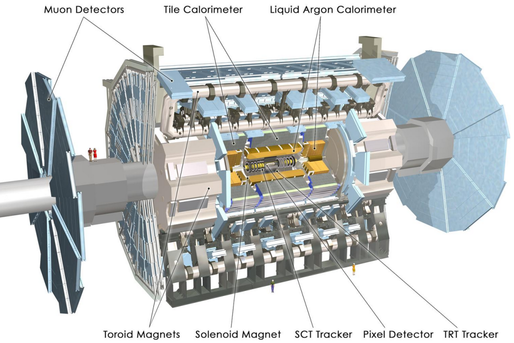
\includegraphics[width=0.49\linewidth]{images/ATLAS.png}
    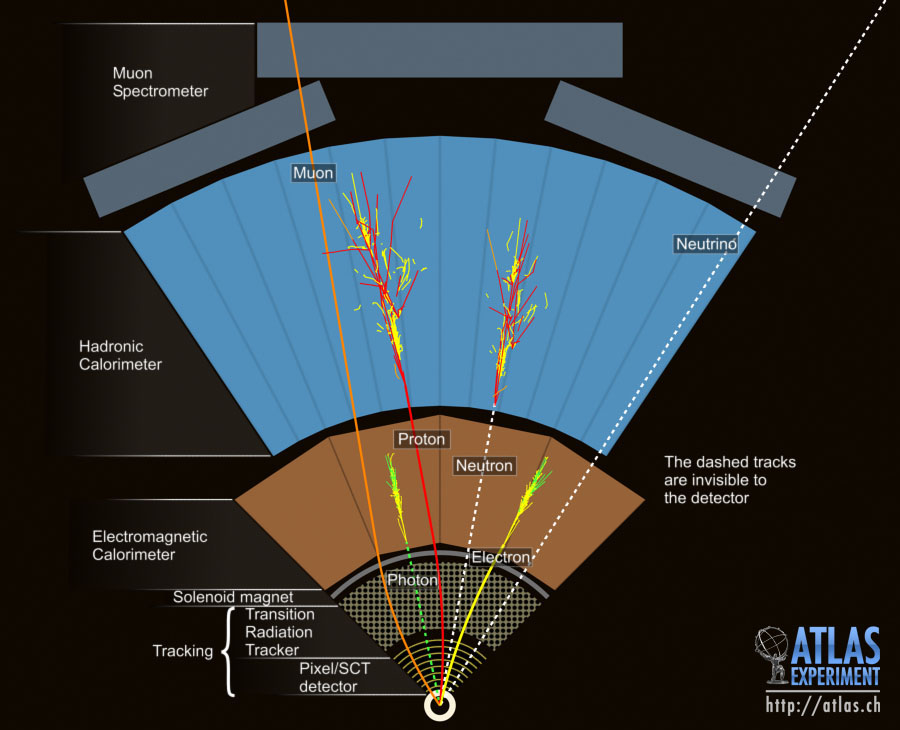
\includegraphics[width=0.41\linewidth]{images/ATLASinteractions.jpg}
    \caption{(left) A labeled diagram of the ATLAS detector. (right) Interactions of different types of particles in ATLAS.}
    \label{ATLAS}
\end{figure}

%\begin{figure}[t]
%    \centering
%    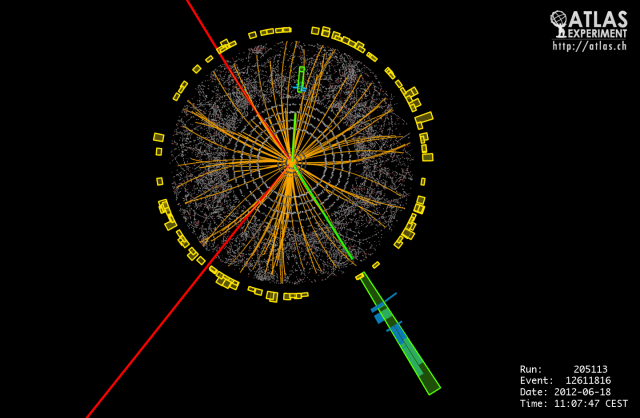
\includegraphics[width=0.5\linewidth]{images/Higgs_2e2mu.png}
%    \caption{A typical reconstructed event display, showing a Higgs boson decaying into two electrons and two muons \cite{Higgs_2e2mu}.}
%    \label{Higgs_2e2mu}
%\end{figure}

\subsection*{Upgrades}

The LHC currently produces about 40 collisions per beam-crossing at 13 TeV center-of-mass energy, but with the proposed high-luminosity LHC (HL-LHC) upgrade there are plans to increase these numbers to 140 collisions per beam-crossing at 14 TeV by 2026, amounting to a total of 250 $fb^{-1}$ of data per year, with ultimate plans to increase to 200 collisions per beam-crossing. During the HL-LHC upgrade, ATLAS similarly plans to upgrade its detection capabilities via the ATLAS Phase-II upgrade, focusing on items such as replacing the inner detector with an all-silicon-based inner tracker (ITk), improving data acquisition, and increasing the granularity of calorimeters \cite{ATLAS_phaseII}. The higher data rates and improved calorimeters provide an incentive to develop and implement the machine-vision based particle identification systems described later in this paper. In the interest of improving upcoming SUSY searches, I have aided in the development of several components in the ATLAS detector. Though they will not be the focus of this paper, as they mostly impact future analyses, I would like to mention them in passing.

First, I worked on investigating methods for improving vertex reconstruction for use in future high-pileup environments, as part of the vertex reconstruction group at ATLAS. The approach we used was based on dividing physical space into a grid of three-dimensional pixels, and using reconstructed tracks to "fill in" those pixels and generate a 3D image. The resulting image was then Fourier transformed, filtered to remove high frequencies, reverse Fourier transformed, and collapsed along the beam axis, resulting in a 1D function where the peaks corresponded to potential vertex locations (vertex "seeds"). Tracks were then associated with their nearest seeds, and from each cluster of tracks we fit a final vertex. I performed performance comparisons between the new and old vertexing methods, and did studies based on tuning parameters of the new method. Some of these results were shown in my presentation at the 2015 ATLAS CP Tracking Workshop \cite{vertex}. I also performed studies on using machine-learning methods to better associate tracks with vertex seeds, and to recognize and recombine "split" vertices, though these methods did not show significant improvements over baseline during my time with the project.

I also performed some work on upgrades to the ITk for the ATLAS Phase-II upgrade. Recently I spent a year at Argonne under the guidance of Dr. Jessica Metcalfe working on manufacturing methods for mass production of silicon pixel detectors in preparation for the upgrade. During that time I worked on setting up a manufacturing lab and various electronic test environments, on assembling pixel modules using various mechanical epoxy-based techniques, on designing adapter boards for readout electronics, and on performing tests on assembled modules. I also participated in a three-month testbeam at Fermilab with the University of Geneva, during which we gathered and analyzed data from a proposed HVCMOS pixel detector. The idea behind this detector was that due to advances in silicon sensor manufacturing, we could build readout circuitry directly into the detector, removing the need for an external readout chip. This resulted in less detector material, and also reduced manufacturing cost. I presented results from this testbeam at DPF 2017 \cite{DPF}, and this analysis, combined with additional data taken by the University of Geneva at the SPS in CERN, will be presented in an upcoming paper on the new detector.

Furthermore, I have contributed some work to the fast tracker (FTk) upgrade for ATLAS \cite{FTk}. The FTk is an FPGA-based method for performing online track reconstruction, for use in the inner detector. I worked on the extrapolator board with Professor Mark Neubaeur's team. The extrapolator is responsible for reconstructing 12-layer tracks (for the 12 layers of the inner detector) using preliminary 8-layer tracks and a collection of hits from the other 4 layers. I developed a new memory storage mechanism for organizing and retrieving hits, and have recently completed a rewrite of the extrapolation code. We are currently working to ensure uninterrupted data flow, and are attempting to optimize our firmware to run at 200 MHz.

%A timeline of the past and future of the LHC is shown in <figure>.
%\begin{figure}[t]
%    \centering
%    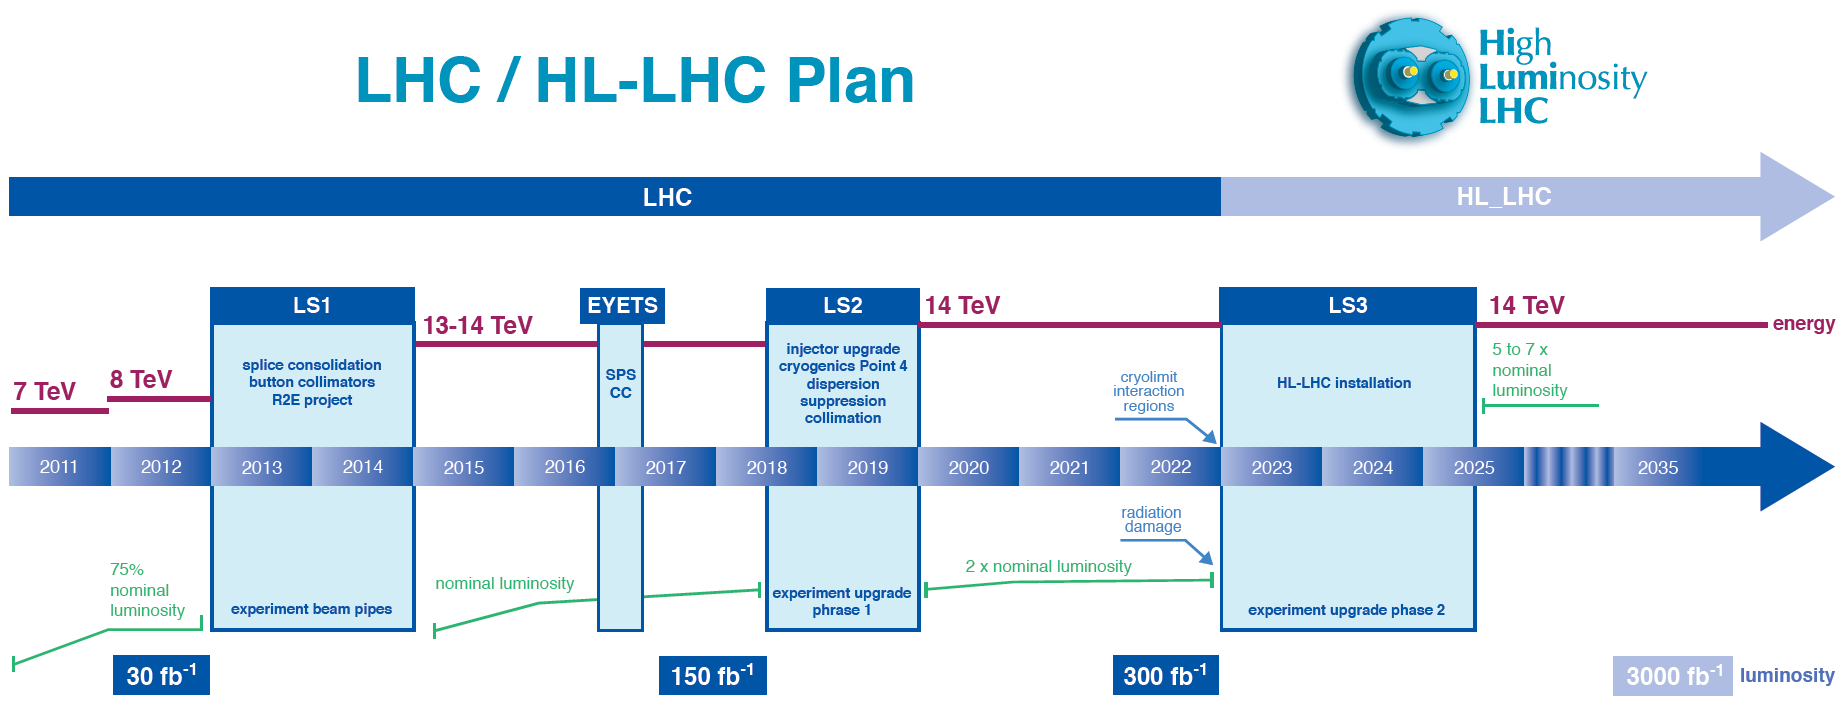
\includegraphics[width=0.7\linewidth]{images/HL-LHC.png}
%    \caption{A timeline of proposed upgrades to ATLAS.}
%    \label{HL-LHC}
%\end{figure}

\section*{THE STANDARD MODEL AND SUSY}

The purpose of the LHC and other similar colliders is to study physics at the most fundamental level of existence. We are interested in probing and measuring the smallest building blocks of nature, and in discovering how they go together. The most complete picture which we have to date is shown on the left side of Figure~\ref{SUSY}. In this model, known as the standard model, we describe the universe as a composition of leptons, quarks, and force carriers. Leptons include the well-known electron, as well as its nearly-invisible partner, the electron neutrino. Quarks include the building blocks of protons and neutrons, the up and down quarks. Furthermore, there are the heavier generations of these particles, which are just like the electron, electron neutrino, up quark, and down quark, only with more mass. We also have the force carriers (or gauge bosons) - photons for the electromagnetic force, gluons for the strong force, and W and Z bosons for the weak force. Finally, completing the picture is the recently-discovered Higgs boson, an excitation of the Higgs field which gives mass to the other fundamental particles. There are also the antimatter counterparts to these particles, which have opposite charge, though the neutral force carriers are their own antiparticles.

%\begin{figure}[t]
%    \centering
%    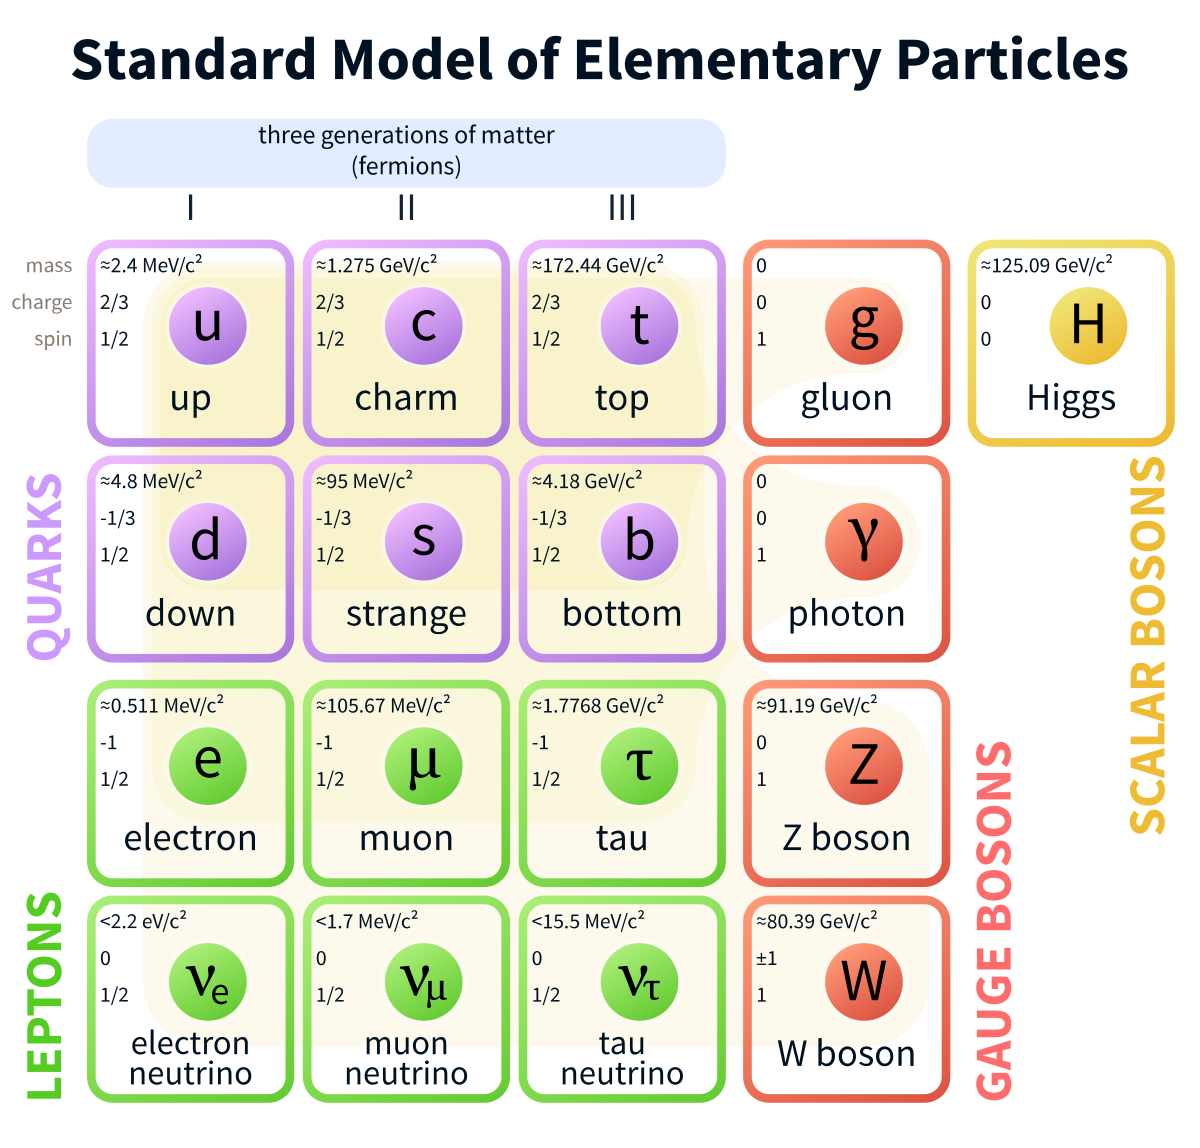
\includegraphics[width=0.7\linewidth]{images/standard_model.png}
%    \caption{The standard model.}
%    \label{standard_model}
%\end{figure}

\begin{figure}[t]
    \centering
    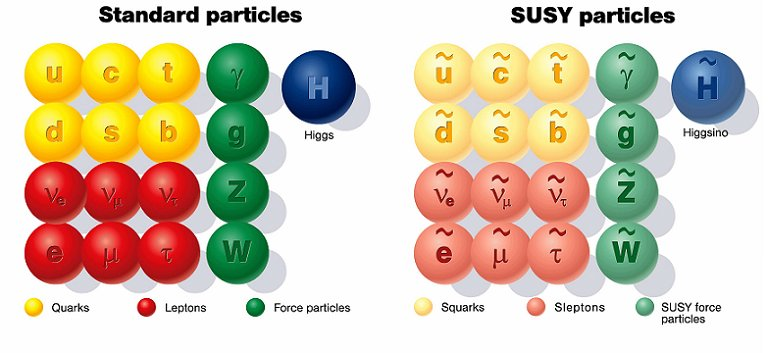
\includegraphics[width=0.7\linewidth]{images/SUSY.png}
    \caption{(left) The standard model. (right) Supersymmetric partners of standard-model particles. This diagram displays the squarks, sleptons, and gauginos which make up SUSY. The gauginos (from top to bottom, and left to right) are the gluino, photino, zino, the winos, and the Higgsinos. The photino, zino, and two neutral Higgsinos combine to form mass eigenstates $\tilde{\chi}^0_1, \tilde{\chi}^0_2, \tilde{\chi}^0_3, \tilde{\chi}^0_4$, which are called the neutralinos. The winos and two charged Higgsinos combine to form $\tilde{\chi}^\pm_1, \tilde{\chi}^\pm_2$, the charginos.}
    \label{SUSY}
\end{figure}

This model has produced some of the most accurate agreements between theory and experiment ever achieved in science, but we know that it does not describe the entire universe. For instance, the standard model only describes ordinary matter and antimatter, but these only account for about $5\%$ of the mass in the universe. Another $27\%$ is dark matter, and the remaining $68\%$ is dark energy. Gravity is not included in the standard model, as it remains the least-understood fundamental force. Many questions about it remain to be answered, such as why gravity is so much weaker than all the other forces. There is also the Higgs hierarchy problem, which relates to why the Higgs boson has the mass that it does \cite{hierarchy}. If we calculate the expected mass of the Higgs, we find that quantum loop corrections from virtual particles ought to push the mass up to an order of magnitude around the breakdown point of known physics, the Planck mass at $m_{Planck} = 10^{18}$ GeV. One way the Higgs can have a mass around 126 GeV is for bosonic and fermionic loop corrections to the Higgs mass (which have opposite sign) to cancel each other out.

Supersymmetric (SUSY) theories have been proposed as a potential solution to some of these problems. According to SUSY (Figure~\ref{SUSY}), there is an additional supersymmetric partner to each particle that we currently know of. Each boson has a fermionic superpartner, and each fermion has a bosonic superpartner. This provides a natural solution to the hierarchy problem. Furthermore, if the lightest neutral SUSY particle is prohibited from decaying into a normal-matter state, it could remain undetected and thus form the basis of dark matter. In addition, if SUSY is imposed as a local symmetry, supergravity theories can be formed, merging the standard model and general relativity.

With all of these strong points, it would seem that SUSY is a very promising theory. However, despite our best efforts, attempts to search for SUSY particles have so far proved unfruitful. Clearly, if SUSY is a correct theory, it must undergo spontaneous symmetry breaking which changes the masses of the undiscovered superpartners. Thus it may be that the undiscovered particles are currently outside the energy range of our colliders (though there are upper limits to particle masses before the theory becomes unnatural), or it may be that the particles are too close together in mass, in which case their decay products will be hard to detect. This second possibility will be examined later in the paper, and will form part of the motivation for developing a low-energy particle identification system.

\section*{A SEARCH FOR SUSY IN 2L2J EVENTS}

Previously, I participated in a search for SUSY, targeting the events shown in Figure~\ref{SUSY_2l2j}. In these events, an initial gluon decays into a $\tilde{\chi}^0_2$ (second-lightest neutralino) and two quarks. The $\tilde{\chi}^0_2$ further decays into $\tilde{\chi}^0_1$ (lightest neutralino) via either a Z boson decay or an intermediate slepton decay. The Z may be either on or off shell. To target these decays, we looked for events with final states containing a same-flavour opposite-sign lepton (electron or muon) pair, two or more jets, and large missing transverse momentum ($E_T^{miss}$). To differentiate between the different models (on-shell Z, off-shell Z, and slepton decay), we looked at the final dilepton mass distribution, as seen in Figure~\ref{mll}. These searches used $\sqrt{s}$ = 13 TeV collision data with an integrated luminosity of $14.7 fb^{-1}$, gathered by the ATLAS detector during 2015 and 2016.

\begin{figure}[t]
    \centering
    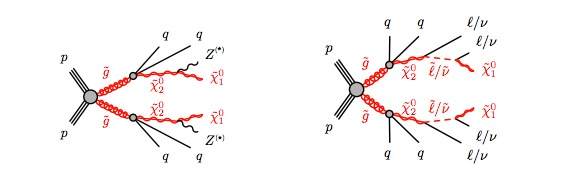
\includegraphics[width=0.7\linewidth]{images/SUSY_2l2j.png}
    \caption{SUSY models involving final states with two leptons, two jets, and large transverse missing energy. Note that though these diagrams show two gluino decay branches, the final state we searched for only required one.}
    \label{SUSY_2l2j}
\end{figure}

\begin{figure}[t]
    \centering
    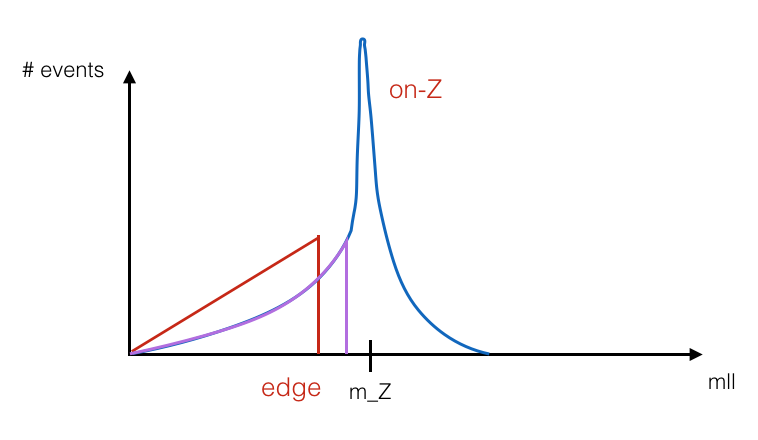
\includegraphics[width=0.5\linewidth]{images/mll.png}
    \caption{Different dilepton mass ($m_{ll}$) distributions. On-shell Z bosons have an $m_{ll}$ peak around the Z mass at 91 GeV, but off-shell Z's would see a sharp cutoff in the $m_{ll}$ distribution at an energy equal to $m_{\tilde{\chi}^0_2} - m_{\tilde{\chi}^0_1}$. Events which went through the slepton decay process would see an entirely different $m_{ll}$ distribution shape.}
    \label{mll}
    
    \centering
    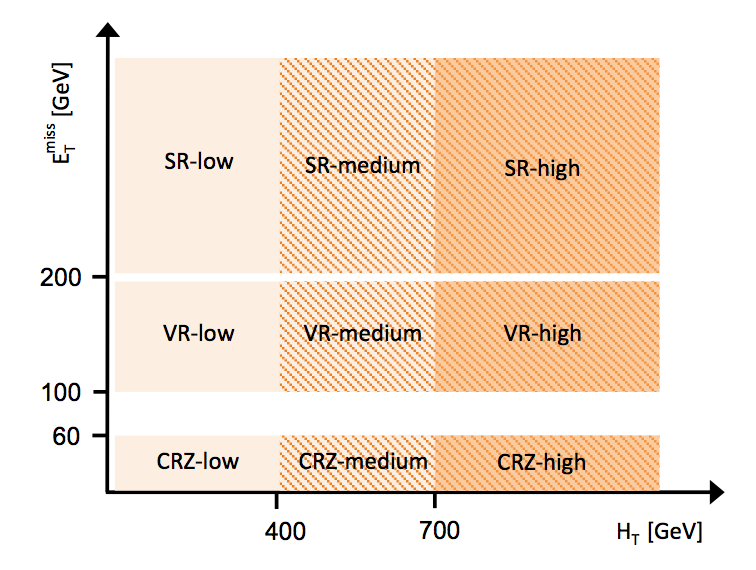
\includegraphics[width=0.45\linewidth]{images/slepton_signal_regions.png}
    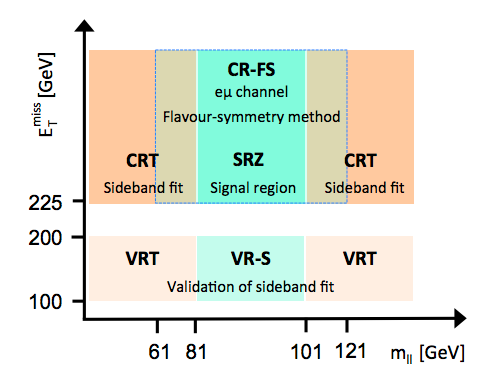
\includegraphics[width=0.45\linewidth]{images/Z_signal_regions.png}
    \caption{Signal regions chosen to maximize signal-over-background ratios given various sparticle masses. The signal regions on the left are for slepton and off-shell Z models, and correspond to low, medium, and high values of $m_{\tilde{\chi}^0_2} - m_{\tilde{\chi}^0_1}$. The signal region on the right is for the on-shell Z model. $H_T$ refers to the total transverse momentum of jets.}
    \label{signal_regions}
\end{figure}

When selecting objects for this analysis, we decided to use signal leptons with transverse momentum ($p_T$) above 25 GeV, and jets with $p_T$ above 30 GeV. For the purposes of performing jet overlap removal and calculating $E_T^{miss}$, we also allowed baseline leptons above 10 GeV and baseline jets above 20 GeV. In the interest of keeping this paper at a reasonable length, the complete set of object selection and triggering criteria will not be included, but can be found in the complete SUSY analysis paper at \cite{SUSY_2l2j}.

As with most high-energy physics searches, there were a variety of standard-model processes which mimicked the final state we were looking for. Of these, the $t\bar{t}$ process was the largest, followed by diboson (WZ/ZZ) processes. Events with a single Z and two or more jets from initial-state radiation could also mimic our signal, provided that mismeasurement of the jet momentum resulted in a large $E_T^{miss}$ for the event. Events from single-top-quark processes and from lepton misidentification also contributed to the background. To accurately model these backgrounds, we used flavor-symmetry, Z/$\gamma^*$, Monte Carlo, and fake estimation methods, all of which will be described below.

As we had several unknown masses in our models, we needed to find multiple signal regions which could optimize the signal-to-background ratio for a variety of different $\tilde{\chi}^0_1$, $\tilde{\chi}^0_2$, and $\tilde{g}$ masses. In Figure~\ref{signal_regions}, we show the four signal regions we chose, along with their associated validation and control regions, which were used to implement and test various background-rejection methods.

\subsection*{Flavor Symmetry}

Flavor symmetry (FS) was an important background rejection method, and removed contributions from processes such as $Z\rightarrow\tau\tau$, $t\tilde{t}$, WW, and tW. Unlike our signal models, which produced only pairs of same-flavor leptons, these processes could produce same-flavor and opposite-flavor lepton pairs with equal probability. The basic idea was to take the opposite-flavor $e\mu$ events from data in each signal region, and to use them to estimate the number of same-flavor events from FS sources in each of those regions. Due to differences in detection and triggering efficiencies for electrons and muons, we had to apply the scaling factor shown in the following equation, where $\epsilon_{e/\mu}$ was the offline selection efficiency for each lepton and $\epsilon_{e\mu/ee}^{trigger}$ was the dilepton trigger efficiency for each channel. The equation for the $\mu\mu$ channel followed the same logic.

\begin{gather}
%n_{ee}^{measured} = n_{ee}^{truth}\epsilon_e^2\epsilon_{ee}^{trigger} \\
%n_{e\mu}^{measured} = n_{e\mu}^{truth}\epsilon_e\epsilon_{\mu}\epsilon_{e\mu}^{trigger} \\
n_{ee}^{measured} = \frac{1}{2}\frac{\epsilon_e}{\epsilon_{\mu}}\frac{\epsilon_{ee}^{trigger}}{\epsilon_{e\mu}^{trigger}}n_{e\mu}^{measured}
\end{gather}

\subsection*{Z/$\gamma^*$ + Jets}

Another important background was single-Z events with two additional jets from initial state radiation. There was no real missing energy in these events, but they could appear to have $E_T^{miss}$ due to mismeasurement of jet momentum. Jets were difficult to model accurately in Monte Carlo simulation due to the complexity of hadronic showering, so to estimate Z + jets, we used a data-driven method where we selected for a similar background ($\gamma$ + jets), and applied reweighting and momentum smearing. Since in this case both $\gamma$ and $Z\rightarrow ll$ were well-measured particles recoiling against two jets, the kinematics of both processes were very similar. One difference came from the fact that $\gamma$ is massless, which caused its $p_T$ distribution to be different from that of Z. We had to correct for this by reweighting $\gamma$ events in bins of $p_T$. Photon $p_T$ also had to be smeared to match the resolution of muon $p_T$ in the $Z\rightarrow\mu\mu$ channel.

%There were also differences in resolution, since photons and electrons were measured quite accurately, but muons had worse resolution, especially at high $p_T$. Thus, to account for the fact that $Z\rightarrow\mu\mu$ events had worse resolution, photon $p_T$ had to be smeared to match the resolution of Z $p_T$ in the $\mu\mu$ channel.

%\begin{figure}[t]
%    \centering
%    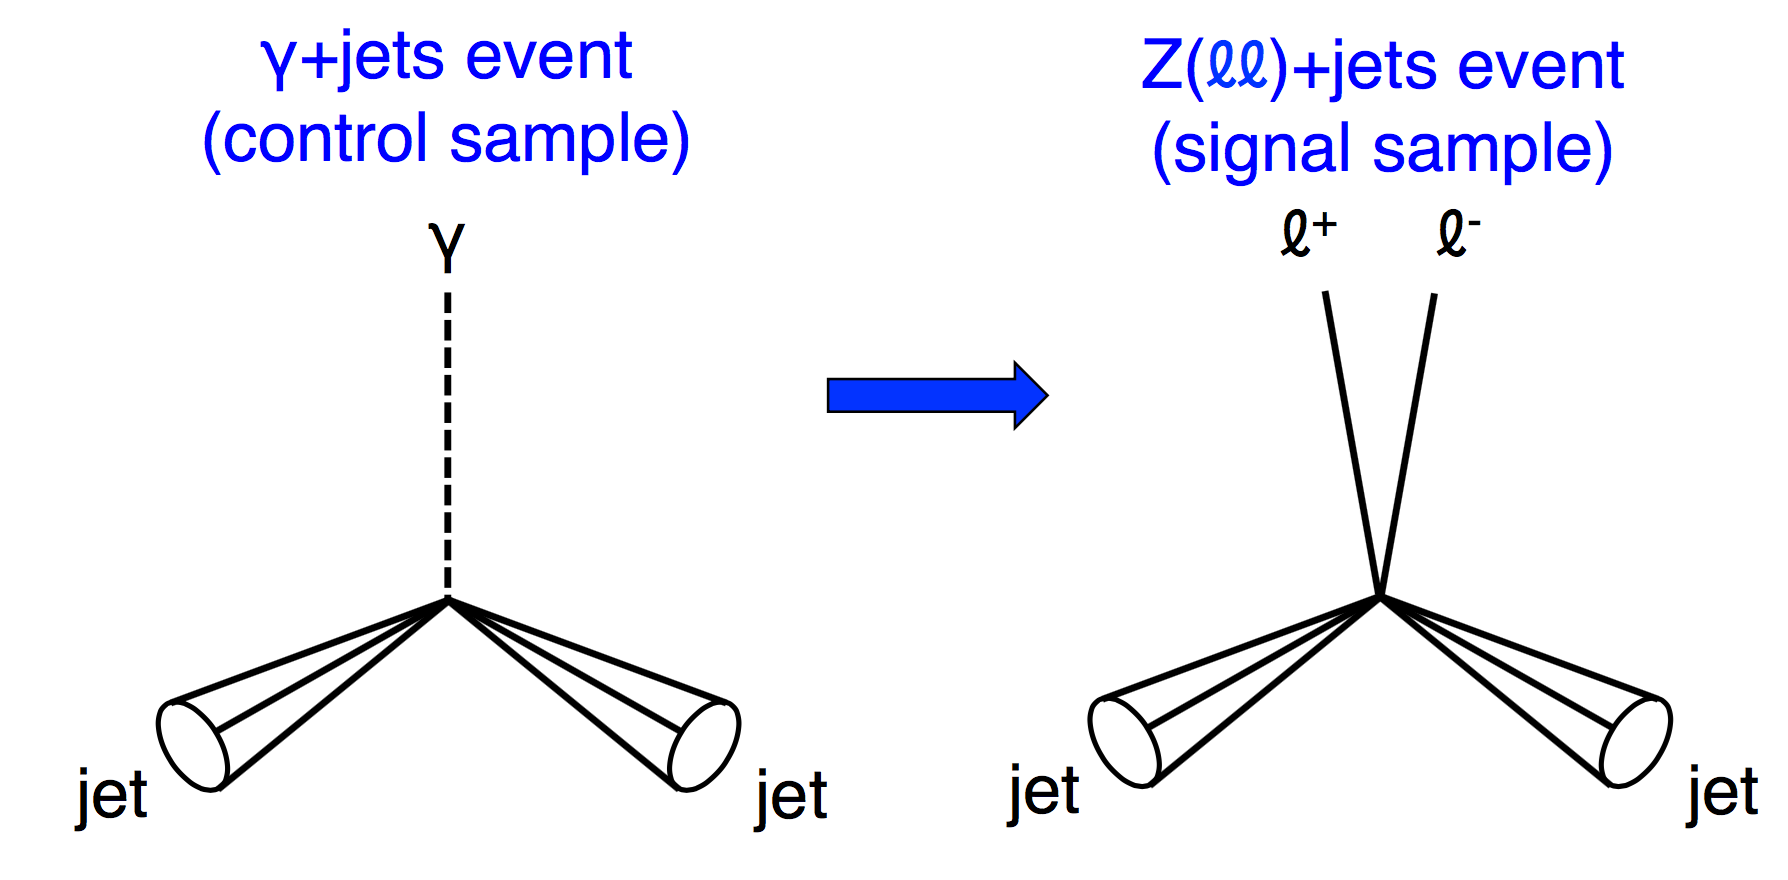
\includegraphics[width=0.8\linewidth]{images/gamma_jets.png}
%    \caption{We selected events in data with $\gamma$ + jets and no leptons (left), and used them to estimate the background contribution from Z + jets (right).}
%    \label{gamma_jets}
%\end{figure}

\subsection*{Fake Leptons}

Another contribution to background came from events where one or more non-leptonic objects were incorrectly identified as leptons. Semileptonic $t\bar{t}$, W + jets, and single top events were included in this category. We estimated the number of fake leptons in each region using a matrix method described in detail in \cite{fake_method}. The general idea was that in each signal region, we would apply both loose and tight lepton selections. We labeled the number of baseline (loose) leptons which passed the signal (tight) cut as $N_{pass}$, and called the ones which failed $N_{fail}$. Given two further numbers, $\epsilon^{real}$ and $\epsilon^{fake}$ (fractions which pass the signal cut), we could then estimate the number of fake signal leptons using the following equation. $\epsilon^{real}$ and $\epsilon^{fake}$ were calculated via a tag-and-probe approach. Expanding this method to a dilepton system (where either or both leptons could be fake) required only that we extend this logic to a 4x4 matrix.

\begin{equation}
N_{pass}^{fake} = \frac{N_{fail}-(1/\epsilon^{real}-1)\times N_{pass}}{1/\epsilon^{fake}-1/\epsilon^{real}}.
\end{equation}

%Using this equation required that we obtain good estimates for $\epsilon^{real}$ and $\epsilon^{fake}$. We could find $\epsilon^{real}$ by looking in a signal region which selected for a high concentration of likely $Z\rightarrow ll$ events, and by performing a tag-and-probe method with the leading lepton as the tag. We estimated $\epsilon^{fake}$ in a similar way, by looking in a region with high likelihood of fake leptons (requiring exactly two same-sign leptons), and using the lower-$p_T$ lepton to calculate $\epsilon^{fake}$. For the fake-lepton region, we made sure to disregard same-sign dilepton events which came about as a result of prompt lepton production. These processes were simulated in Monte Carlo, and subtracted from the data. Expanding this method to a dilepton system (where either or both leptons could be fake) required only that we extend this logic to a 4x4 matrix. Fake lepton rates were calculated in $p_T$ bins for each region.

\subsection*{Monte Carlo}

Finally, we come to the section that I was responsible for, the Monte Carlo simulation of diboson events, mainly $WZ\rightarrow lll\nu$ and $ZZ\rightarrow ll\nu\nu$, as well as the simulation of smaller diboson processes and other rare events such as ttZ, ttW, ttWWW, etc. Modeling for the two major diboson components (which make up about $20-30\%$ of the background in each region) was validated in three regions, VR-WZ, VR-ZZ, and VR-3L. VR-WZ and VR-3L were both intended to validate the WZ process, just in different regions of phase space. VR-ZZ was a four-lepton region meant to validate the $ZZ\rightarrow llll$ process, taking advantage of similarities in the MC simulation process for $ZZ\rightarrow ll\nu\nu$ and $ZZ\rightarrow llll$. These regions were all chosen to be above $90\%$ pure in diboson processes. Data-MC comparisons of $E_T^{miss}$, $H_T$, jet multiplicity, and boson $p_T$ in these regions showed good agreement, demonstrating that there were no difficulties with QCD modeling. Particular attention was paid to MC simulation of jet parameters, and differences between Powheg and Sherpa-generated samples for each region were included in the systematic errors.

The Powheg generator had better jet-modeling properties overall. However, due to the way Powheg produced $ll\nu\nu$ samples, the $WW\rightarrow ll\nu\nu$ and $ZZ\rightarrow ll\nu\nu$ processes could not be separated at the truth level. Since the WW process was already included in the flavor-symmetry method, we had to remove it in order to avoid double-counting. To do this, we estimated the ZZ component in each region by subtracting the DF component of $VV\rightarrow ll\nu\nu$ from the SF component. Since the ZZ process is expected to be much greater than the WW component only in the on-Z $m_{ll}$ region, we calculated systematics for this method by taking the off-Z $m_{ll}$ component of each region and checking the exactness of SF and DF cancellation.

\subsection*{Results}

Results for each signal region are shown in Figure~\ref{results}. The on-Z region shows a significance of $0.47\sigma$, and the largest local significance in any slepton region is $1.7\sigma$. Based on these results, we obtain the exclusion contours in Figure~\ref{exclusion}. In conclusion, this search found only results consistent with the standard model. As seen from the exclusion plots, we have two possible avenues to consider if we wish to extend this search. We can either go towards the higher-mass region, or we could look at the compressed-mass region where mass differences between SUSY particles are very small.

\begin{figure}[t]
    \centering
    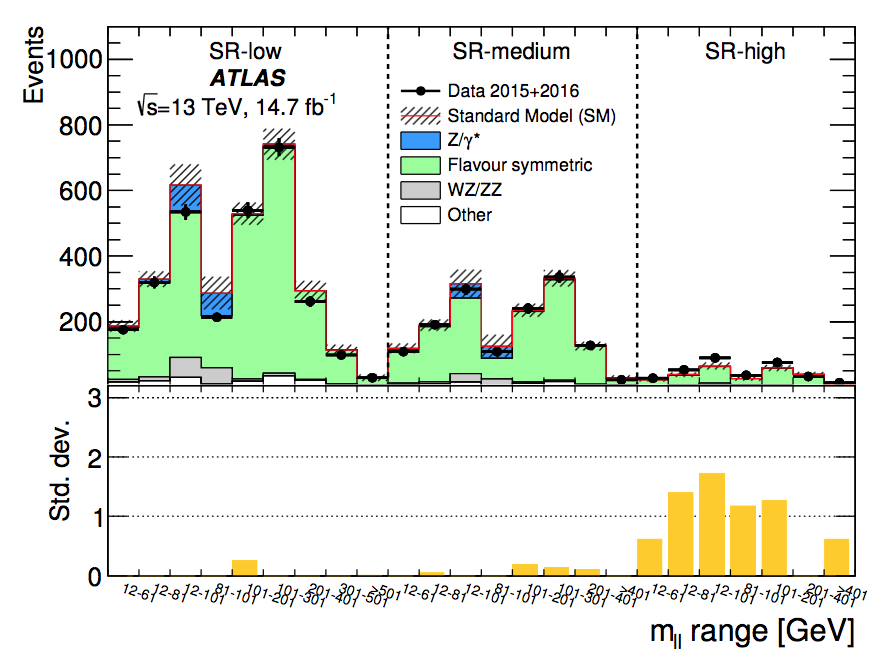
\includegraphics[width=0.4\linewidth]{images/slepton_results.png}
    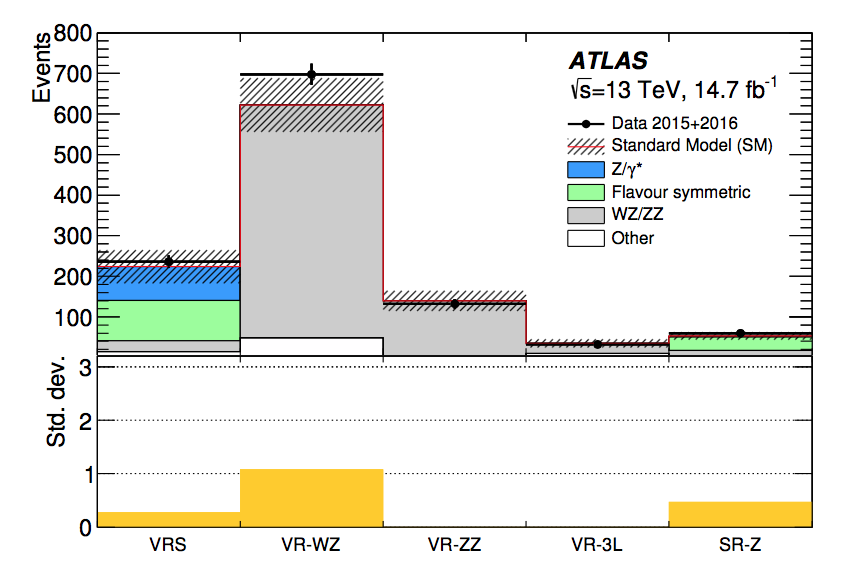
\includegraphics[width=0.45\linewidth]{images/on-Z_results.png}
    \caption{(left) Data-MC comparisons for slepton models. (right) Data-MC comparisons for on-Z model.}
    \label{results}
\end{figure}

\begin{figure}[t]
    \centering
    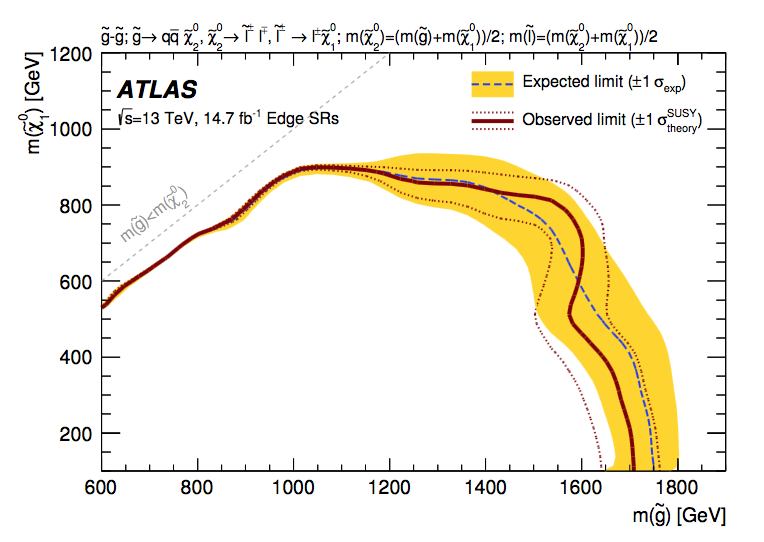
\includegraphics[width=0.45\linewidth]{images/slepton_exclusion.png}
    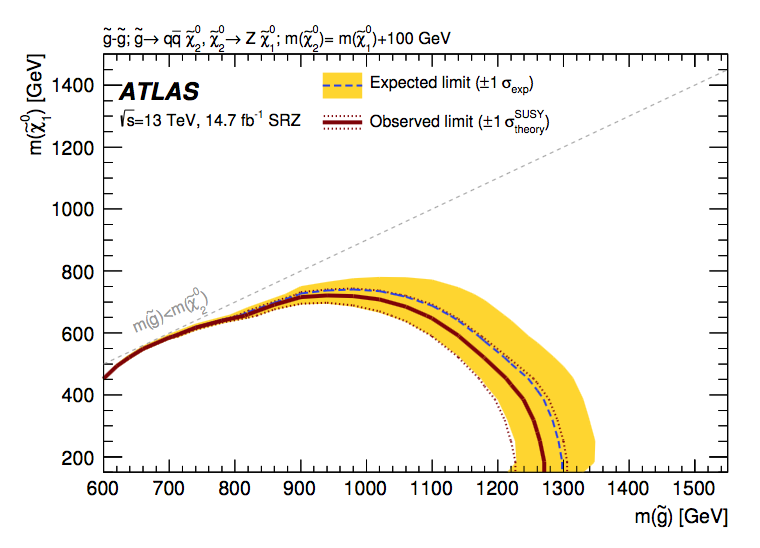
\includegraphics[width=0.45\linewidth]{images/on-Z_exclusion.png}
    \caption{(left) Exclusion contours in $m_{\tilde{\chi}_1^0}$, $m_{\tilde{g}}$ space for slepton models where $m_{\tilde{\chi}_2^0} = \frac{1}{2}(m_{\tilde{g}} + m_{\tilde{\chi}_1^0})$. (right) Exclusion contours for on-Z models where $m_{\tilde{\chi}_2^0} = m_{\tilde{\chi}_1^0} + 100$ GeV.}
    \label{exclusion}
\end{figure}

There are good theoretical reasons to look at the compressed-mass region. As mentioned previously, the SUSY gauge particles combine into mass eigenstates called the neutralinos ($\tilde{\chi}^0_{1,2,3,4}$) and charginos ($\tilde{\chi}^\pm_{1,2}$). Together, all these particles are collectively known as electroweakinos. The neutralinos are formed from the photino, zino, and neutral Higgsinos, where the photino and zino are themselves mixtures of the bino and neutral wino. The charginos are formed from the charged winos and charged Higgsinos. If we consider a situation (motivated by naturalness arguments) where the Higgsino mass is close to the weak scale, but the masses of the bino and wino are much higher \cite{Higgsino}, then the lightest electroweakinos ($\tilde{\chi}^0_1, \tilde{\chi}^0_2, \tilde{\chi}^\pm_1$) would be dominated by Higgsino contributions, and in this case their masses would be separated in the range of hundreds of MeV to tens of GeV, putting the model outside the exclusion limits of our previous search.

A previous search using the Higgsino model excluded (with $95\%$ confidence) next-to-lightest neutralino masses of up to 130 GeV, and down to mass splittings of 3 GeV \cite{Higgsino}. Since this model involves very soft (low-pT) leptons, we can improve the sensitivity of the search if we created a more accurate method of identifying and measuring particles at low energy. One way we can improve upon traditional particle identification techniques is to make use of new methods in machine learning and image recognition on raw detector data. An approach for developing such a tool will be described in the following sections. After building the tool, we aim to enhance the search using ATLAS data gathered through the end of LHC Run II (about 100 $fb^{-1}$).

\section*{MACHINE LEARNING}

Machine learning is an area of computer science in which we attempt to create intelligent systems that are able to make complex, human-level decisions. It has seen use in recent years in areas as diverse as self-driving cars, language processing, and automatic crop harvesting. In recent years, many machine learning techniques have started being applied to the realm of high-energy physics. Due to very high volumes of data production, especially for planned next-gen colliders such as the HL-LHC, and due the complexity involved in reconstructing each collision event, machine learning has been applied to applications such as track reconstruction, vertex-finding, and jet identification, and was used in the Higgs discovery. The field is extremely broad with many applications, so I will only attempt to describe a few basic ideas here.

Boiled down to its fundamentals, the goal of a machine learning process is  to take a set of input data, and to generate the optimal outputs. For instance, a facial recognition system may take as its inputs a set of pixels originating from a camera or video feed, and output a pointer to a name in a database of people. A translation program may take a string of characters in one language as text input and output another string in a different language. A drone with obstacle avoidance may take input from visual systems and from mounted sensors, and output instructions to its various motors. Even an organic entity takes chemical, physical, and internal inputs from its environment, and outputs chemical and electrical signals to its muscles and organs. There are two major classifications of machine-learning algorithms. One type is supervised, where a system is fed a series of training examples, and is told explicitly what type of output the system should be attempting to obtain for each example. This is the case for an image-classification algorithm, which may be fed many different input images, along with labels for each image. The other major type of machine learning algorithm is unsupervised. In this case, the algorithm is still fed input data, but is not told what the output should be. This is generally the case for clustering algorithms, such as those used for data compression and error/outlier detection.

To build a particle recognition system, we will eventually require unsupervised learning in order to implement systems that recognize and zoom in on energy clusters. However, in the interest of conciseness, I will focus only on supervised algorithms here. As its name suggests, the field of machine learning is generally focused on how to get an algorithm to "learn" from input data. In a supervised learning example, the algorithm takes the form of a complicated expression with many tunable parameters. This expression may be in the form of a series of matrix operations, or as a chain of cut-based classifiers, or in general any other form of an input-output system with tunable components. This algorithm begins with some initialized parameters, and is fed a chunk of input data (which may be composed of one or several input examples). The algorithm then spits out its outputs, which are compared to the correct outputs. The accuracy of the response is then quantified using a "loss function", which in practice is often either the L2 distance, the logistic loss function, or the cross entropy loss. I will now talk about two very common algorithms, the boosted decision tree (BDT) and neural net (NN).

\subsection*{BDT}

Simply speaking, a decision tree is simply a series of branching paths based on input data, which one can follow to reach a conclusion. An example of a very simple decision tree is shown in Figure~\ref{decision_tree}. Decision trees are similar to how objects and signal regions are selected in a traditional high-energy-physics analysis. For example, one may ask whether an event has more than, less than, or equal to three leptons. If the event has exactly three leptons, one may ask whether the top two leptons have dilepton mass within a certain range, etc. Based on these decisions, an experimenter can decide what signal region an event belongs in. As another example, imagine that we are trying to determine what kind of particle we have seen in an event. We could ask whether the particle left a track in the inner detector, whether the amount of energy it deposited in the calorimeter is in a certain range, etc. Given a random ordered set of input variables, an optimal decision tree can be calculated for decisions made in that specific order.

A boosted decision tree is created by combining many different decision trees together \cite{BDT}. Any given decision tree can be very weak, containing only a small number of branches and a small maximum depth. However, by taking the weighted results of many decision trees together, we can get a more accurate result than can be achieved by any single tree. For the sake of space, the AdaBoost BDT training algorithm will not be discussed here.

\begin{figure}[t]
    \centering
    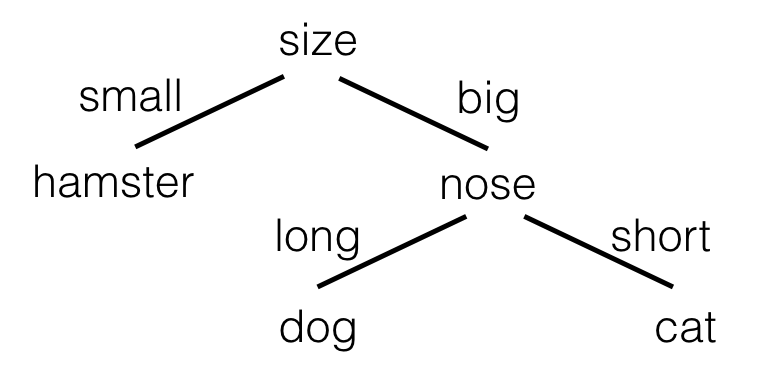
\includegraphics[width=0.5\linewidth]{images/decision_tree.png}
    \caption{An example of a decision tree that a child may use to classify a household pet.}
    \label{decision_tree}
\end{figure}

\subsection*{Neural Net}

A neural net is a machine learning architecture based on the physical structure of neurons in the human brain \cite{neural_net}. The basic unit of a neural net is a neuron, which has a numerical value, one or more inputs, and one or more outputs. These neurons are connected together so that the output of one neuron becomes the input of one or more other neurons. Here we will only consider simple feed-forward neural nets, where all the inputs to a neuron come from neurons closer to the beginning of the net, and all the outputs of that neuron go to neurons nearer the end of the net. That is, there are no "loops", and there are no connections between neurons at the same depth. The input values for an event form the first layer of neurons, and the output is derived from the last layer. Each link between neurons is associated with a "weight", or multiplicative constant. Each neuron is also associated with a "bias", or an additive constant. Letting $y_i$ be the value of the $i^{th}$ neuron, $w_{i,j}$ be the value of the weight between neurons $i$ and $j$, and $b_i$ be the bias associated with neuron $i$, we see that the value of a neuron is equal to $y_j = \sum{w_{i,j}y_i} + b_j$. Each neuron is also typically followed by a nonlinear "activation" function, so that the result of the entire net is not simply equivalent to a single matrix operation on the input. We see then that for a given set of weights and biases, we can calculate the output value for a net given any inputs.

In order to train a neural net, we use "back-propagation", meaning that for each event (or set of events) we perform gradient descent on each weight and bias in order to minimize the resulting loss function. Over the course of many events, the net can fall into a state where it produces the correct outputs with high accuracy. In this way, the neural net training is simply a form of function optimization. Many important topics, such as how to weight initialization, methods of gradient descent, net architectures, etc. will not be discussed in this paper.

\begin{figure}[t]
    \centering
    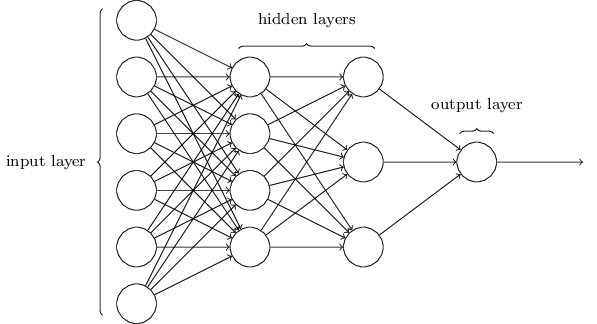
\includegraphics[width=0.5\linewidth]{images/neural_net.png}
    \caption{A diagram showing a typical densely-connected neural net.}
    \label{neural_net}
\end{figure}

\section*{MACHINE LEARNING FOR PARTICLE IDENTIFICATION}

The next generation of detectors currently under development often feature an increase in granularity of the electromagnetic and hadronic calorimeters. This is true of the ATLAS Phase-II upgrade, and also of the highly granular CALICE sampling calorimeter proposed for the ILC, which was used for the initial studies presented in this section. These improved detector designs provide an excellent opportunity for applying machine learning algorithms for identifying particles and measuring their energies.

Our purpose in this experiment is to create a neural-net classifier using calorimeter data, which can demonstrably perform better on object identification than traditional feature-based analysis techniques can. Specifically, we have chosen to build two classifiers - one to distinguish between electrons and charged pions, and one for photons and neutral pions. In order to create a more challenging classification task, we have chosen only pion events which are likely to be confused with either electrons or photons. For charged pions, this meant taking events where the total energy deposited in the ECAL was at least 40 times greater than the energy deposited in HCAL. For neutral pions, this meant taking events where pions decayed into two photons with an opening angle of less than 0.01 radians.

The study is based on pseudo-data simulated with GEANT4 in the proposed Linear Collider Detector (LCD) for the CLIC accelerator~\cite{Lebrun}. Though we intend to extend our studies to the ATLAS detector for use in Higgsino searches, the complicated non-uniform accordion-shaped calorimeters in ATLAS add some difficulties to the task. In contrast, the LCD has uniform calorimeter cell sizes, which makes it a good starting point. The calorimeter in this detector consists of a regular grid of 3D cells with cell sizes of 5.1 mm$^3$ and an inner calorimeter radius of 1.5 m. In this dataset, individual electron, photon, charged pion, and neutral pion particles are shot orthogonally into the calorimeter surface. The particle energy is set to a fixed value of 60 GeV. For each event, a 25x25x25 cell slice of the electromagnetic calorimeter (ECAL) and the corresponding 5x5x60 cell slice of the hadronic calorimeter (HCAL) are stored as two 3D arrays of deposited energy in each cell.

We use BDT's as a proxy for traditional feature-based analysis on calorimeter data. This provides a baseline against which to compare the results of neural net performance. All features used in the BDT are calculated using traditional methods, where the complete list of features we use is as follows: total energy deposited in ECAL, total number of hits registered in ECAL, the ratio of energy deposited in ECAL first layer over energy deposited in second layer, the ratio of energy deposited in ECAL first layer over all ECAL energy, 2nd through 6th moments in the x, y, and z dimensions for ECAL energy deposits, all equivalent features for HCAL, ratio of HCAL to ECAL energy, and ratio of number of hits in HCAL to ECAL. We also examined the effect of several n-subjettiness measures, mostly to help distinguish between photons and neutral pions. Specifically, by measuring how well energy depositions were described as belonging to either one, two, or three jets, we hoped to distinguish between single photons and pions which had decayed into two photons. However, n-subjettiness was computationally expensive to calculate and did not result in much classification improvement, so its usage was dropped.

Initial studies on different net architectures showed no significant differences in performance between convolutional neural nets (CNN's) and simply-connected dense neural nets (DNN's). Therefore, we chose to focus only on DNN's, due to the smaller number of hyperparameters we would have to scan over. In the nets we trained, the ECAL and HCAL inputs were separately flattened and fed into two cell-based DNN's with identical architectures, and the outputs were merged before applying a softmax layer and computing categorical cross-entropy loss. We used two different types of nets - one based on raw cell energy inputs, and one based on the same input features that we had calculated for the BDT. This was to investigate whether differences in performance between the BDT and DNN could be attributable simply to a difference in architecture, without any actual additional information processing. Because neural nets are sensitive to the scale of input data, for the feature-based neural net we first normalized each feature by calculating the z-score for each event (i.e. $\frac{x-\bar{x}}{std(x)}$).

Each two-object classification dataset was divided into 400,000 training and 100,000 test events. After performing hyperparameter scans on Blue Waters, we decided on a DNN architecture consisting of 4 hidden layers with 256 neurons each, ReLU activation, and dropout of 0.5, trained with Adam optimization with a learning rate of 0.001. A BDT hyperparameter scan yielded best performance with 400 estimators, maximum depth of 5, and learning rate of 0.5. In our studies, we found that the most powerful feature-based discriminators are the second $x$ and $y$ moments, which measure the lateral shower width. Performance curves for the BDT's and DNN's are shown in Figure~\ref{ROCs}, and performance values are shown in Table~\ref{AUCs}.

\begin{figure}[!t]
    \centering
    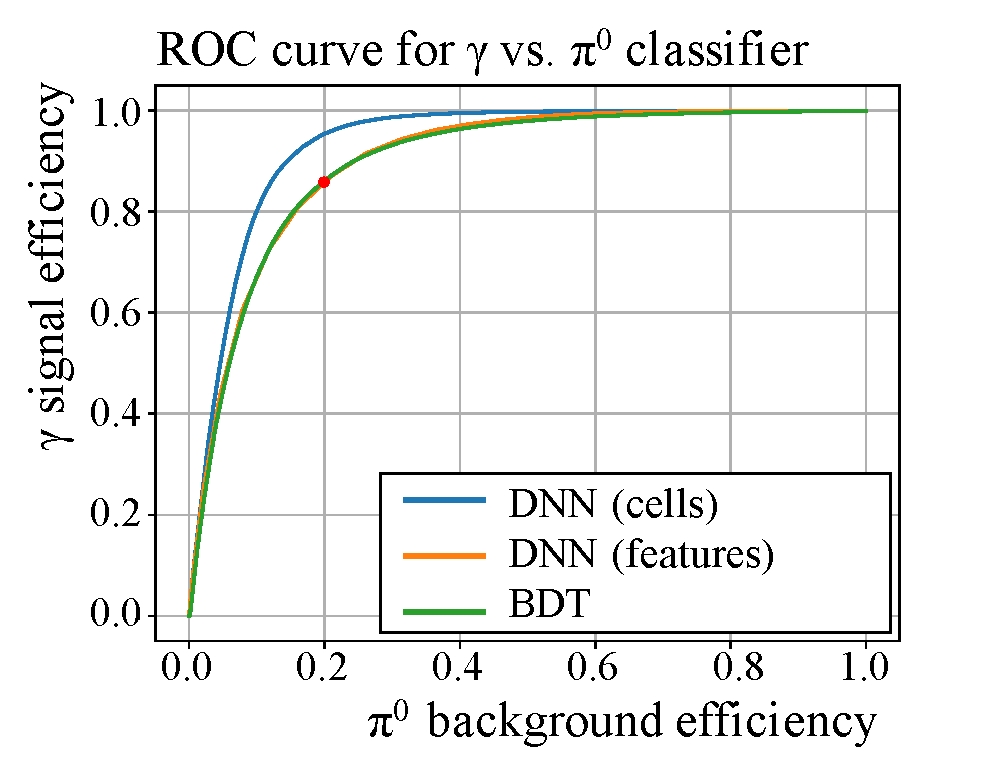
\includegraphics[width=0.33\linewidth]{images/photon_pi0.pdf}
    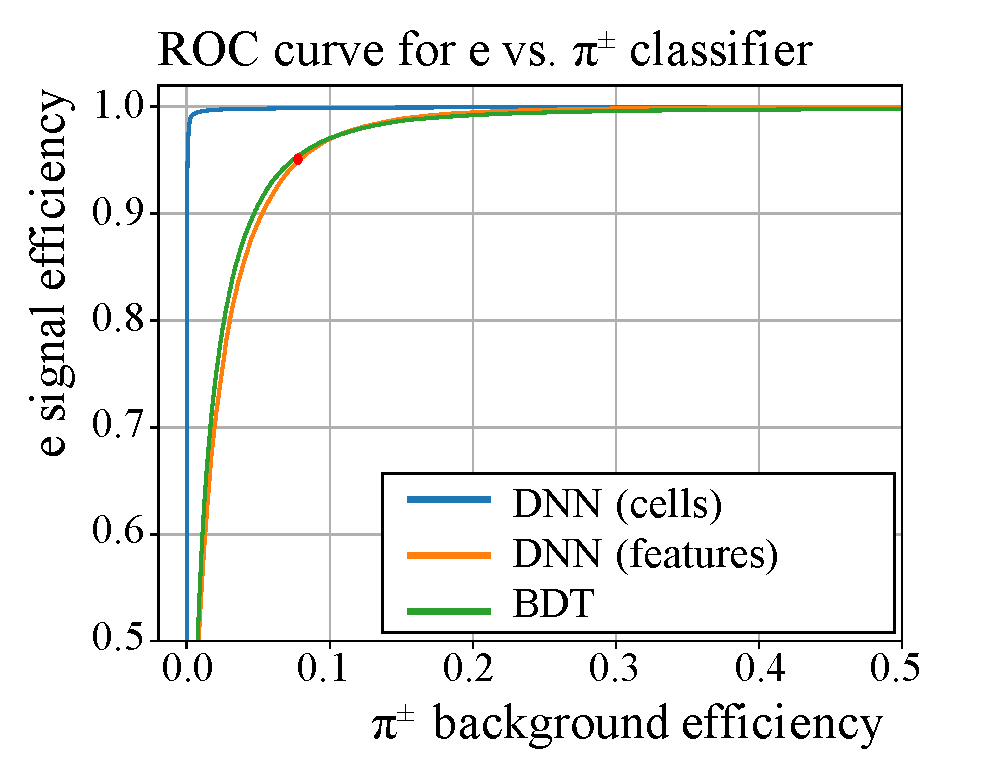
\includegraphics[width=0.33\linewidth]{images/electron_chpi.pdf}
    \caption{Signal vs. background efficiency ROC curves for the (left) $\gamma$ vs. $\pi^0$ and (right) $e$ vs. $\pi$ classifier. The red dots mark the chosen BDT working point.}
    \label{ROCs}
\end{figure}

\begin{table}[!ht]
    \centering
    \begin{tabular}[!t]{l|cccc|cccc}
        \hline
        & \multicolumn{4}{c}{\textbf{$\gamma$ vs. $\pi^0$}} & \multicolumn{4}{c}{\textbf{$e$ vs. $\pi$}}\\
        \hline
        \textbf{Model} & \textbf{acc.} &  \textbf{AUC} & \textbf{$\Delta \epsilon_{\mathrm{sig}}$} & \textbf{$\Delta R_{\mathrm{bkg}}$} & \textbf{acc.} &  \textbf{AUC} & \textbf{$\Delta \epsilon_{\mathrm{sig}}$} & \textbf{$\Delta R_{\mathrm{bkg}}$} \\
        \hline
        \centering
        BDT & 83.1\% & 89.8\% & - & - & 93.8\% & 98.0\% & - & - \\
        DNN (features) & 82.8\% & 90.2\% & 0.9\% & 0.95 & 93.6\% & 98.0\% & -0.1\% & 0.95 \\
        DNN (cells) & 87.2\% & 93.5\% & 9.4\% & 1.63 & 99.4\% & 99.9\% & 4.9\% & 151 \\
        \hline
        \hline
    \end{tabular}
    \vspace{5pt}
    \caption{Performance parameters for BDT and DNN classifiers.} 
    \label{AUCs}
\end{table}

The areas under curve (AUC) and accuracies (acc.)
for the cell-based DNNs are significantly better than for the feature-based DNNs and BDTs (which both have similar performance). This demonstrates that the DNN is able to extract additional information from the calorimeter data which is not captured via traditional measures. Choosing the working point on the BDT ROC curve indicated in Figure~\ref{ROCs}, we obtain the following improvement metrics for the cell-based DNN. For the $\gamma$ vs. $\pi^0$ ($e$ vs. $\pi^\pm$) classifier, the cell-based DNN may be used to either increase the signal efficiency by $\Delta \epsilon_{\mathrm{sig}} = \epsilon_{\mathrm{sig}}^{\mathrm{DNN}} - \epsilon_{\mathrm{sig}}^{\mathrm{BDT}}=9.4$\% (4.9\%) for fixed background efficiency, or decrease the background efficiency by a factor $\Delta R_{\mathrm{bkg}} = \epsilon_{\mathrm{bkg}}^{\mathrm{BDT}} / \epsilon_{\mathrm{bkg}}^{\mathrm{DNN}}= 1.6$ (151) for fixed signal efficiency.

\section*{FUTURE WORK}

We have shown that neural nets are capable of outperforming traditional feature-based analyses on lepton identification tasks. Our colleagues working with us have also shown good machine-learning results for particle energy identification, and for generative adversarial network (GAN) based approaches for rapid simulation of lepton showers in simulation. Going forward, our next steps are to perform classification on a range of particle energies, rather than simply at a fixed 60 GeV, especially focusing on lower energy scales. We would also like to implement clustering and attention algorithms, which would allow us to zoom in and perform classification on individual particles in a multi-particle event. After that, the next step is to translate this work into the ATLAS detector geometry. We may do this via the use of deep belief nets. The ultimate goal is then to use the resulting tool to help identify leptons in a Higgsino search for new physics beyond the standard model.

\begin{thebibliography}{9}

\bibitem{ATLAS_website} 
ATLAS Detector and Technology,
\\\texttt{https://atlas.cern/discover/detector}

%\bibitem{Higgs_2e2mu}
%ATLAS Collaboration.
%Event display of a H to 2e2mu candidate event,
%\\\texttt{https://cds.cern.ch/record/1459500}

\bibitem{ATLAS_phaseII}
ATLAS Phase-II Upgrade Scoping Document,
\\\texttt{https://cds.cern.ch/record/2055248/files/LHCC-G-166.pdf}

\bibitem{vertex} 
ATLAS Vertex Reconstruction Group.
\textit{New Seed Finding Method in Run II Vertexing}.
Presentation at ATLAS CP Tracking Workshop, Nov 30, 2015.

\bibitem{DPF} 
Zhang, M.
\textit{Track Reconstruction Efficiencies with the H35DEMO HV-CMOS Pixel Detector}.
Presentation at DPF 2017, July 31, 2017.

\bibitem{FTk}
Shochet et al.
\textit{Fast TracKer (FTK) Technical Design Report}.
CERN-LHCC-2013-007.
\\\texttt{https://cds.cern.ch/record/1552953}

\bibitem{hierarchy} 
Stephen Martin. 
\textit{A Supersymmetry Primer}. 
\\\texttt{arXiv:hep-ph/9709356}

\bibitem{SUSY_2l2j}
ATLAS Collaboration.
\textit{Search for new phenomena in events containing a same-flavour opposite-sign dilepton pair, jets, and large missing transverse momentum in $\sqrt{s}$ = 13 TeV $pp$ collisions with the ATLAS detector}.
ATLAS-CONF-2016-098.
\\\texttt{https://cds.cern.ch/record/2217165}

\bibitem{fake_method}
ATLAS Collaboration.
\textit{Search for squarks and gluinos in events with isolated leptons, jets and missing transverse momentum at $\sqrt{s}$ = 8 TeV with the ATLAS detector}.
JHEP 04 (2015) 116.
arXiv: 1501.03555 [hep-ex].

\bibitem{BDT}
Robert E. Schapire.
\textit{Explaining AdaBoost}.
\\\texttt{http://rob.schapire.net/papers/ explaining-adaboost.pdf}

\bibitem{neural_net}
Michael A. Nielsen.
\textit{Neural Networks and Deep Learning}.
Determination Press, 2015.

\bibitem{Lebrun}
Lebrun, P. et al.
\textit{The CLIC Programme: Towards a Staged e+e- Linear Collider Exploring the Terascale : CLIC Conceptual Design Report}.
10.5170/CERN-2012-005.

\bibitem{Higgsino}
ATLAS Collaboration.
\textit{Search for electroweak production of supersymmetric states in scenarios with compressed mass spectra at $\sqrt{s}$ = 13 TeV with the ATLAS detector}.
ATLAS-SUSY-2016-25-002.
\\\texttt{https://cds.cern.ch/record/2292513}

\end{thebibliography}

\end{document}
